\documentclass[12pt, a4paper, twoside]{article}

%% Preamble
\usepackage{umatfgspanish}
\usepackage{tabto}
\newcommand\ttab{\tab \hspace{-5cm}}
\graphicspath{{./images/}}

\begin{document}
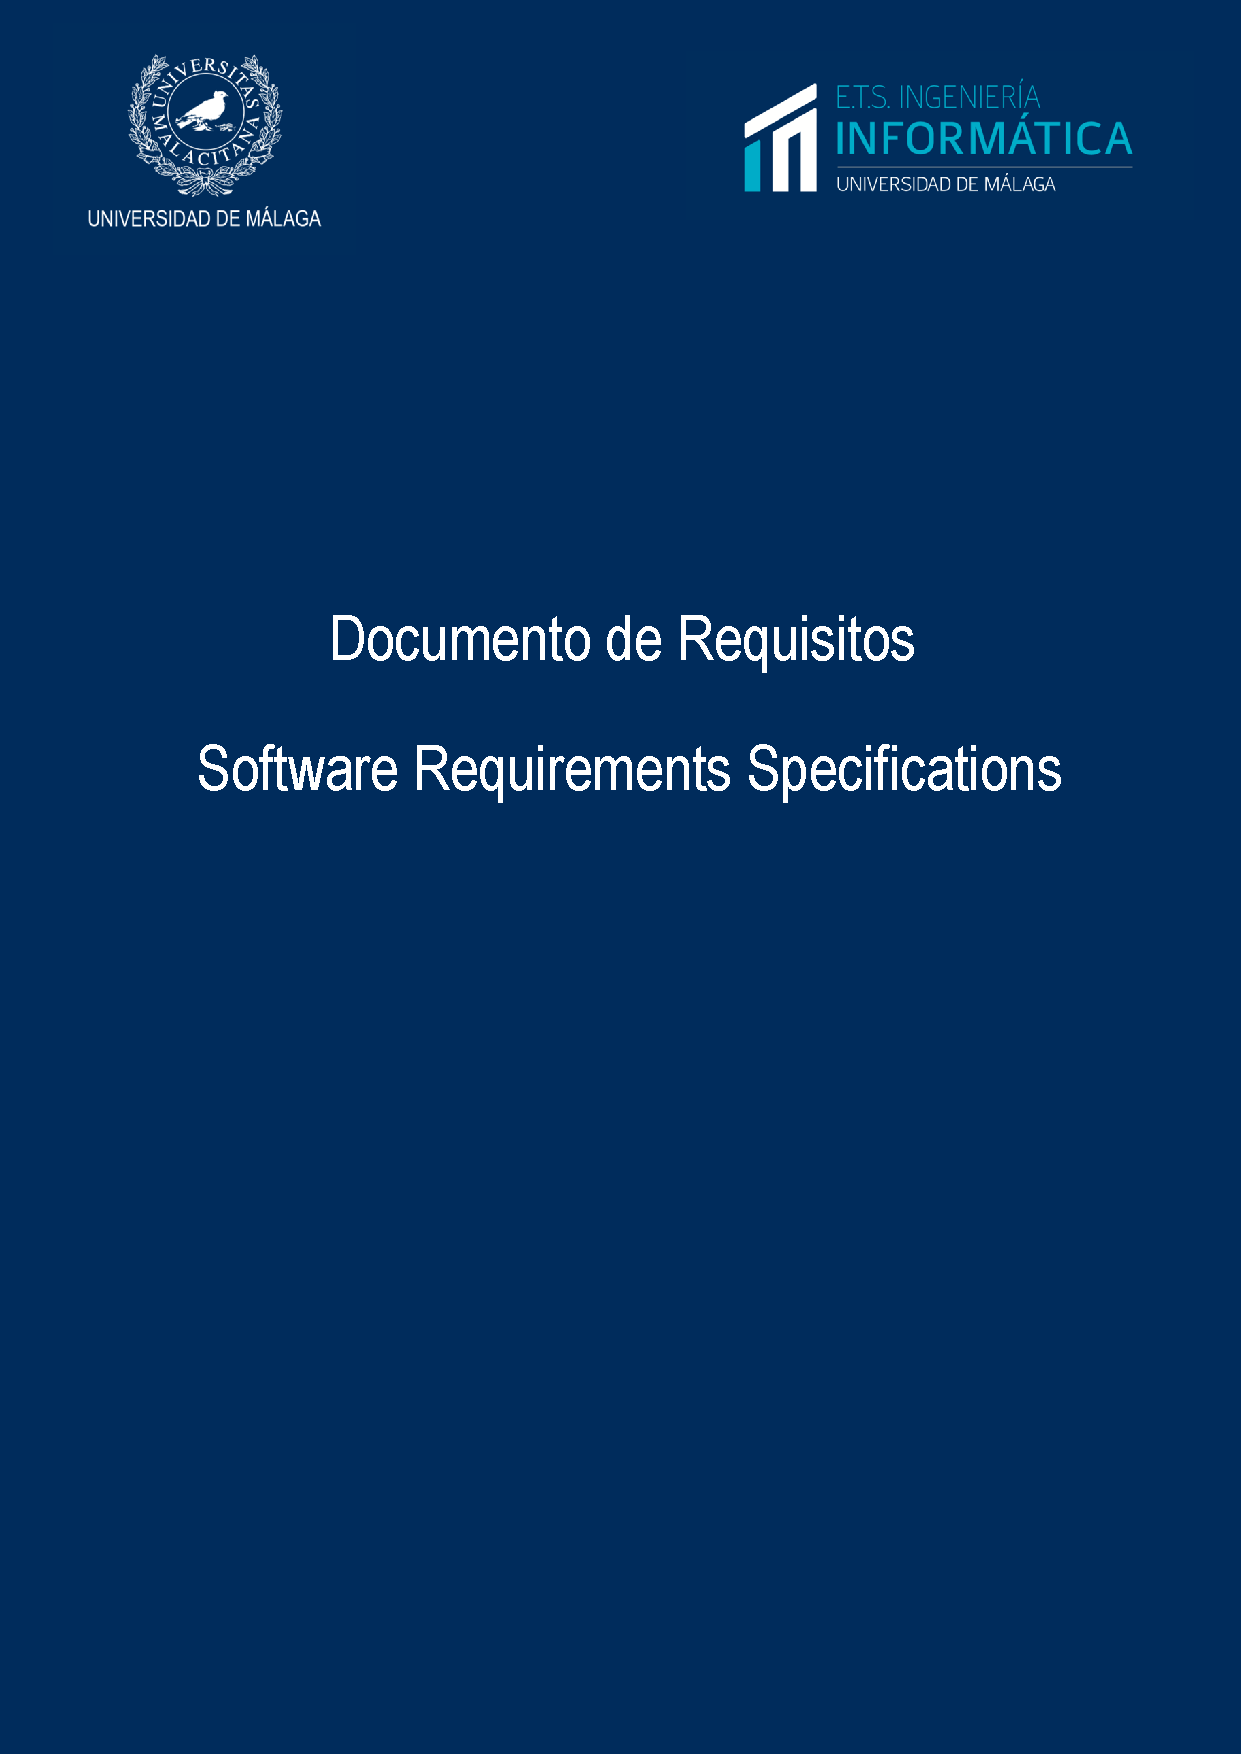
\includepdf[noautoscale=true, width=\paperwidth]{title.pdf}
\newpage
\tableofcontents

%% Sections
\section{Introducción}
\subsection{Propósito}
Desarrollar una plataforma virtual común que permita:
\begin{itemize}
  \item Gestionar y organizar la información de cualquier edificio 
        dentro de una ciudad.
  \item Interconectar cualquier elemento integrable a la red de Internet 
        (dispositivos IoT) que se encuentren en un edificio (Smart Building)
        usando interfaces de comunicación que ya son estándar.
\end{itemize}

\subsection{Ámbito}
Debido a las características del software que hacen uso de las tecnologías 
``Internet de las Cosas'' (IoT) para la gestión de dispositivos conectados a
la red de un Edificio Inteligente (Smart Building), se ha decidido darle el nombre de
``IBuilding''.

% META
IBuilding pretende ser un gestor de los edificios de una ciudad con el que
poder consultar información sobre ellos y manipular sus dispositivos.
 
 % OBJETIVO
Para ello, IBuilding deberá almacenar datos de los edificios y 
deberá disponer de herramientas para acceder y manipular los dispositivos que se instalen
en los mismos.

% Beneficio
De esta manera, se puede enriquecer el valor de una ciudad, permitiendo digitalizar más
datos sobre ella y poder generar una información más fiel y útil para que otras personas
y servicios digitales puedan hacer uso de ella.

IBuilding dispondrá de un servidor central (llamado DataBuilding) que, usando la tecnología
de Fiware, almacenará los datos propios de cada edificio (como la ubicación o el 
tipo de servicio que ofrecen) y los dispositivos disponibles en el mismo. 
Se podrán consultar los datos a través de una API que usará modelos estándares 
de datos.

Los diferentes dispositivos necesitarán controladores que permitan conectarse
a internet para poder manipularlos mediante algún API.

Como ejemplo se desarrollarán algunos Controllers, para hacer uso y alimentar a la API.
Estos dotarán a los dispostivos (Ya sean físicos o virtuales) de acceso a internet, usando interfaces 
estándares, como UltraLight 2.0, OneM2M o directamente NGSI-LD. Ejemplos de Controllers podrían
ser SensorController o ANNPlateController.

El desarrollo de una interfaz de usuario puede ser útil para la gestión de la plataforma
a nivel usuario. Es por eso que también habrá un frontal para hacer uso de IBuilding
que se conectará al DataBuilding y podrá visualizar/modificar los datos oportunos.
Para referirnos a este frontal usaremos el nombre de FrontalBuilding.

\section{Visión general del producto}
\subsubsection{Perspectiva del Producto}
Desde el punto de visto externo, IBuilding puede ser visto como un servicio de integración que
\begin{itemize}
  \item ofrezca datos sobre los edificio a aplicaciones terceras.
  \item permita controlar dispositivos mediante una API estándar y conocida.
  \item permita conectar dispositivos IoT de la Smart Building a la red.
\end{itemize}

Para la implementación de esta interfaz Fiware es un candidato ideal, ya que ofrece NGSI-LD,
una interfaz de comunicación reconocida por diferentes organismo importantes de referencia en toda la Unión Europea.

Además, Fiware deja abierta la posiblidad de implementar otras interfaces que se usan en desarrollo de dispositivos
IoT como UltraLight 2.0 o OneM2M, que también se considera un estándar reconocido por organismos
como la ETSI.

\begin{figure}[h]
  \centering
  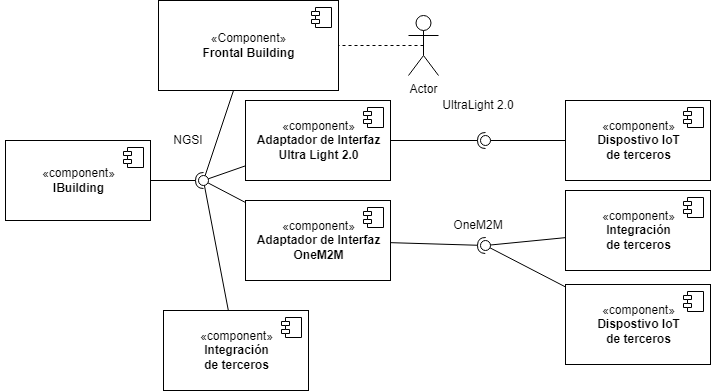
\includegraphics[width=0.8\textwidth]{IBuildingGenericComponents.1.1.png}
  \caption{Niveles de integración posibles siguiendo una aproximación con Gemelo Digital}
\end{figure}

\subsubsection{Interfaces de Usuario}
Se utilizará como guía de diseño Material Design.

Material Design es un ecosistema de diseños desarrollada por Google
que siguen un conjunto de reglas para definir el estilo de la aplicación.

Debido a las características de los usuarios que hacen uso habitual de internet,
aplicar estilos de diseño similares a las de aplicaciones populares puede ayudar a aumentar
el nivel de familiarización e intuitividad de la aplicación (Twitter, Facebook, Google...).

Muchas de las aplicaciones populares hacen uso de esta guía.
Material Design tiene unas especificaciones muy extensas y muy bien definidas. 

\subsubsection{Interfaces Software}
Para poder afirmar que un sistema está impulsado por Fiware, es necesario incluir un Context Broker del catálogo de Fiware.
Se ha elegido Orion-LD Context Broker, por implementar la interfaz NGSI-LD y por sus características de tamaño.

Además, por cuestiones de Seguridad, también se incluirán IdM Keyrock y Wilma, que son softwares completamente integrables y
compatibles con NGSI-LD. 

También se incluirá FogFlow como solución para orquestar flujos de trabajos que involucren a los dispositivos IoT. Esta solución 
se beneficia de la computación en la niebla para optimizar llamadas innecesarias a servidores y ahorrar tiempo y dinero por ahorro
de cómputos en servidores en la nube. Este servicio también tiene compatibilidad con NGSI-LD.

Como último, se incluirán los IoT Agents: Softwares de Fiware que se encargan de adaptar la interfaz NGSI-LD a otros protocolos
e interfaces para poder ampliar las interfaces de comunicación que se ofrecen. Los IoT Agents que se van a incluir en este proyecto
son IoT Agent - Ultralight 2.0 y OpenMTC.
\begin{center}
  \begin{tabular}{ |c|c|c|c|c| } 
   \hline
   Nombre                     & Abreviatura & Última Versión & Interfaz Relevante & Fuente \\ \hline
   Orion-LD Context Broker    & OCB         & 1.1.2          & NGSI-LD            & https://github.com/FIWARE/context.Orion-LD \\ \hline 
   Identity Manager - Keyrock & IdM Keyrock & 8.3.1          & IdM GE API         & https://github.com/ging/fiware-idm \\ \hline
   PEP Proxy - Wilma          & Wilma       & 8.3            & NGSI-LD            & https://github.com/ging/fiware-pep-proxy \\ \hline
   FogFlow                    & FogFlow     & 3.2.8          & NGSI-LD            & https://github.com/smartfog/fogflow \\ \hline
   IoT Agent - Ultralight 2.0 & IotAgentUL  & 1.23.0         & Ultralight 2.0     & https://github.com/telefonicaid/iotagent-ul \\ \hline
   OpenMTC                    & OpenMTC     & 1.3.0          & OneM2M             & https://github.com/OpenMTC/OpenMTC \\ \hline
  \end{tabular}
\end{center}

\subsubsubsection{NGSI-LD}
La interfaz NGSI-LD es muy apropiada para el proyecto. Está estandarizada por la ETSI y
son muchas las aplicaciones de ámbitos inteligentes que lo utilizan.

Tiene una base semántica muy bien definida sobre RDF y Semática Web, e implementa el Linked Data, 
que permite interconectar los recursos por toda la web, por lo que le da más calidad y usabilidad
a los datos.
\subsubsubsection{IdM GE API}
La seguridad en la IoT es un asunto muy crítico, ya que son muchos procesos que se ejecutan automáticamente
desde diversos microservicios y dipositivos que necesitan validar su autenticidad.

Por este motivo se pretende utilizar Identity Manager, que implementa protocolos de seguridad
actuales, como OAuth2.0 para manipular los datos de los usuarios y es compatible con Fiware.
Esta interfaz se utilizará para gestionar la seguridad del sistema.
Se puede consultar su documentación desde los siguientes enlaces: 

https://keyrock.docs.apiary.io/
https://keyrock-fiware.github.io
\subsubsubsection{Ultralight 2.0}
Protocolo orientado a la comunicación entre dispositivos IoT.
Sus características hacen que sea muy ligero y óptimo para el IoT, sobretodo
en escenarios de recursos muy limitados.
Se utilizará para ampliar las interfaces que ofrece el sistema al mundo exterior
para incrementar las opciones de integración con otros dispositivos.

https://fiware-iotagent-ul.readthedocs.io/en/latest/index.html

\subsubsubsection{OneM2M}
Es una organización cuyo objetivo es el de crear un estandar internacional para la interoperabilidad
entre dispositivos físicos e internet.

Con este estándar se pueden orquestar dispositivos IoT de una manera muy eficiente y óptima, además,
también está reconocido por diversos organismos como la ETSII, por lo tanto también es interesante
implementarlo, por su nivel de internacionalización y su verdadera utilidad en la IoT.

\section{Funciones del producto}
Cualquier persona podrá:
 Registrarse y loguearse en la aplicación y podrá visualizar un mapa con los edificios cercanos.
 Listar los edificios con diferentes filtros (tipos de edificio, por distancia, ...)
 Visualizar la información del edificio si tiene permisos.

Creación y configuración del Edificio:
 Un usuario podrá crear edificios. Para ello rellenará un formulario con los datos necesarios que
 tendrán que ser revisado por un adminsitrador del sistema.
 Una vez creado un edificio se podrá gestionar la información del mismo y añadir dispositivos IoT oportunos.

Roles en un edificio:
 Usuarios tendrán roles dentro de un edificio. La información y el uso de los dispositivos a los cuales
 los usuarios pueden acceder se puede configurar por roles.

\begin{figure}[h]
  \centering
  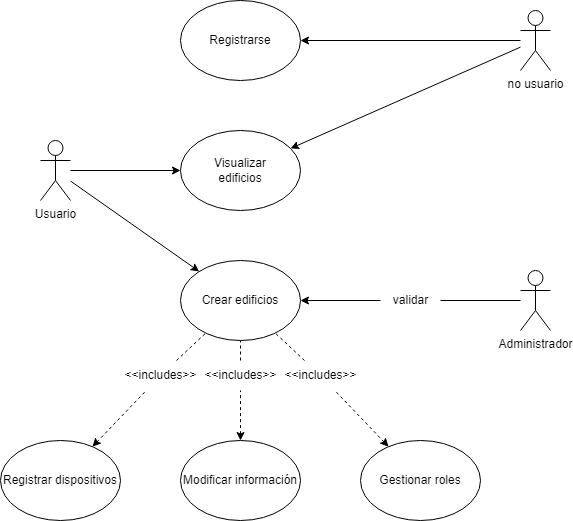
\includegraphics[width=0.8\textwidth]{UserCase.0.1.png}
  \caption{Diagrama de casos de uso}
\end{figure}

 \subsubsection{Características de los Usuarios}
 El usuario objetivo es aquel que vive en ciudades grandes con un nivel tecnológico avanzado,
 por lo tanto, es un usuario familirializado con las tecnologías y que hace un uso
 habitual de internet, en su mayoría.

 El rango incluye usuarios de todas las edades y niveles educativos, que, por lo general
 no tienen un nivel técnico muy avanzado.

 También podemos encontrarnos con un conjunto de usuarios que
 no estén tan habituadas a usar ciertas aplicaciones o que tengan algún nivel de discapacidad
 que dificulte su utilización.

\subsection{Definiciones}
\begin{itemize}
    \item \textbf{Sensores}\ttab Los sensores son dispositivos IoT cuya labor principal es recolectar datos.
    \item \textbf{Actuadores}\ttab Los actuadores son dispositivos IoT cuya función principal hacer una tarea.
\end{itemize}

\section{Referencias}

\section{Requisitos}
\subsection{Requisitos funcionales}
\begin{center}
  \begin{tabular}{ |c|c|c|c|c| } 
  \hline
  ID      & Título & Descripción \\ \hline
  RF-EDI1 & RUD edificios & Se pueden manejar los datos de un edificio. 
    Cualquier usuario podrá visualizar los edificios validados. 
    Los editores y el usuario que envió la solicitud de creación del edificio (creador) podrá editar los datos.
    El creador del edificio o cualquier administrador de la plataforma será el único que podrá borrarlo.  \\ \hline
  % NF: Como lo ordeno, filtros, buscador... Detalles de la vista de detalles del edificio (mapa, salseo...)
  RF-EDI2 & Solicitud de creación de edificio & Cualquier usuario logueado puede solicitar la creación de un edificio rellenando un formulario. Al enviar los datos se insertan en la base de datos con un atributo que indique su estado, quedando solamente visibles para los administradores. \\ \hline
  RF-EDI3 & Aceptar solicitud de creación de edificio & Un administrador podrá aceptar solicitudes de creación de un edificio. Una vez aceptadas cambia el estado a aprobado y pasan a ser visibles para todos los usuarios \\ \hline
  RF-EDI4 & Denegar solicitud de creación de edificio & Un administrador podrá denegar solicitudes de creación de un edificio. Cuando se rechazen, estos se eliminarán de la base de datos. \\ \hline
  
  RF-USU1 & RUD de Usuarios & Los usuarios logueados podrán visualizar los perfiles de otras personas, actualizar sus datos o darse de baja. \\ \hline
  % Voy a utilizar (no me acuerdo como se llama) La cosa esta de auth de fiware.
  RF-USU2 & Registro en la aplicación & Cualquier usuario podrá registrarse en el sistema. \\ \hline 
  RF-USU3 & Validación del acceso & Cualquier usuario registrado podrá iniciar sesión en la aplicación usando las credenciales proporcionadas en el registro. \\ \hline
  % NF: CUALQUIER USUARIO REGISTRADO O NO PODRÁ ACCEDER A LA APLICACIÓN. UN USUARIO NO REGISTRADO ENTRARÁ DE FORMA ANÓNIMA.
  RF-USU4 & Cerrar sesión & Cualquier usuario logueado podrá cerrar sesión. \\ \hline
  % NF: EL TOKEN GENERADO SE GUARDARÁ EN SESSION STGORATE... USARE JSONWEWTOKEN... DURACIÓN DE SESIÓN? 24H? ES PREGUNTA.

  RF-ROL1 & Maestro roles de la aplicación & Hay 3 roles en la aplicación: administrador, usuario y anónimo. \\ \hline
  RF-ROL2 & Maestro roles de un edificio & Cualquier usuario registrado podrá tener 1 rol de los siguientes en cada edificio: creador, editor, miembro, público \\ \hline
  RF-ROL3 & Otorgar rol de edficio & El creador de un edificio podrá otorgar roles en su edificio a cualquier usuario registrado en la aplicación. El criterio para otorgar los roles queda a cargo del creador. \\ \hline

  RF-INI1 & Acceso a la página de inicio & Cualquier usuario puede acceder a la página principal. \\ \hline

  RF-DIS1 & CRUD dispositivos & Dentro de un edificio se podrán incluir dipositivos IoT que interactúen con otros usuarios, entendiendo por 
  interacción la lectura de datos o activarlos para que realicen alguna función.
  El creador o los editores de un edificio podrán añadir, editar o eliminar nuevos dispositivos al mismo. Podrán indicar la visibilidad de los datos: 
  \begin{itemize}
    \item público: Cualquier usuario que acceda al edificio podrá interactuar con el dispositivo.
    \item privado: Solo los usuarios que tengan uno de los siguientes roles: creador, editor o miembro, podrán interactuar con el dispositivo.
  \end{itemize}
  \\ \hline
  \end{tabular}
\end{center}

 \subsection{Requisitos no funcionales}
 \begin{center}
  \begin{tabular}{ |c|c|c|c|c| } 
  \hline
  ID       & Título & Descripción \\ \hline
  RNF-EDI1 & Ordenación en el listado de edificios & Los edificios se ordenarán por cercanía a la ubicación de la persona si se pudiera utilizar.
  En caso de no estar disponible, se ordenará por orden alfabético. \\ \hline

  RNF-EDI2 & Filtrado en el listado de ordenación de edificios & Los edificios se podrán filtrar por nombre, tipo de edificio, distancia o
  si tiene algún rol especial en ese edificio. \\ \hline

  RNF-EDI3 & Detalles de un edificio & Se podrán visualizar los detalles de un edficio. En la vista de los detalles, se incluirá
  un mapa mostrando la ubicación del edificio. \\ \hline
  % NF: Como lo ordeno, filtros, buscador... Detalles de la vista de detalles del edificio (mapa, salseo...)

  RNF-USU1 & Servicio de Autenticación de Fiware & Se utilizarán los microservicios de autenticación de Identity Manager 
  para la autenticación de los usuarios y de los dispositivos en el sistema por compatibilidad con Fiware. \\ \hline
  % Voy a utilizar (no me acuerdo como se llama) La cosa esta de auth de fiware.
  
  RNF-USU2 & Acceso anónimo & Cualquier usuario registrado o no podrá acceder a la aplicación. Un usuario no registrado entrará de forma anónima. \\ \hline
  % NF: CUALQUIER USUARIO REGISTRADO O NO PODRÁ ACCEDER A LA APLICACIÓN. UN USUARIO NO REGISTRADO ENTRARÁ DE FORMA ANÓNIMA.
  
  RNF-USU3 & Token de sesión  & Se utilizará un token de sesión JWT 
   que expirará cada 24 horas
   y que la aplicación guardará en el session storage  \\ \hline
  % NF: EL TOKEN GENERADO SE GUARDARÁ EN SESSION STGORATE... USARE JSONWEWTOKEN... DURACIÓN DE SESIÓN? 24H? ES PREGUNTA.

  \end{tabular}
\end{center}
\section{Apéndice}
\subsection{Acrónimos y Abreviaturas}
\begin{itemize}
    \item \textbf{IoT}\ttab Internet de las Cosas.
    \item \textbf{API}\ttab Application Program Interface.
  \end{itemize}
\end{document}